% !TEX root = ../main.tex
\chapter{Results}


\section{State Machine}
To validate the basic operation of a Python framework that consumed NEM and household data, orchestrated battery charge/discharge and produced results for household cost, a basic state machine was designed as shown in Figure~\ref{fig:state_machine}.

\begin{figure}[H]
    \centering
    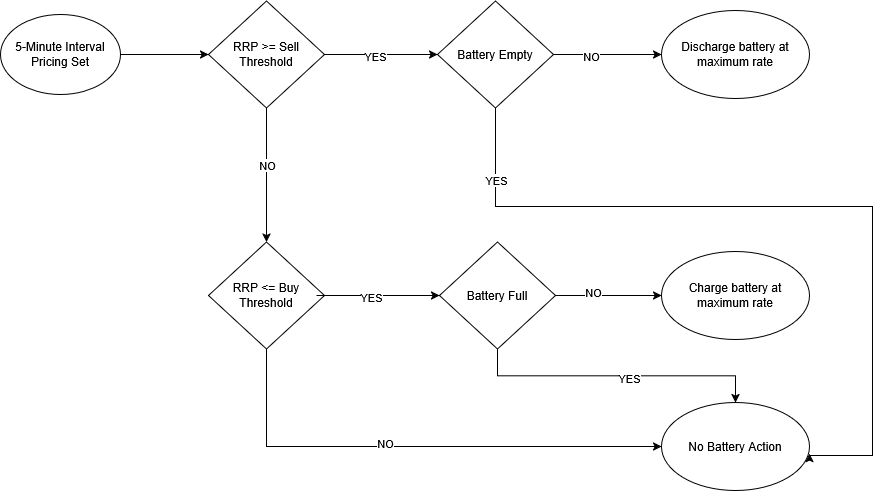
\includegraphics[width=1\textwidth]{images/SimplifiedStateMachineFlowChart.png}
    \caption{A flow chart for state machine trading}
    \label{fig:state_machine}
\end{figure}

The model was trained on a grid search to determine sell thresholds and buy thresholds for a lossless 20 kWh battery with an 11.04 kW inverter, which starts the month empty. Surplus solar may charge the battery at up to 20 kW. A 60x60 grid search was used with buy ranges from \$0/MWh to \$87.50/MWh and a sell range from \$87.50 to \$189.33. The grid value that produced the lowest net-cost to the consumer was selected. 
The grid was searched using data from December 2024 NEM RRP and household import/export data. Dispatch intervals with an RRP outside the 15th to 85th percentile range were removed before the search, which leaves 6256 of the 8928 intervals, and the battery was simulated across the remaining intervals as one continuous series. The net profit reported for the search is therefore the result on that reduced series and not the result for the whole of December. The result of the optimisation is summarised in Table~\ref{tab:optimised_thresholds}.

\begin{table}[H]
\centering
\begin{tabular}{lr}
\toprule
\textbf{Parameter} & \textbf{Value} \\
\midrule
Buy threshold  & \$69.70  \\
Sell threshold & \$127.20 \\
Net profit on the reduced Dec. 2024 series     & \$-34.35 \\
\bottomrule
\end{tabular}
\caption{Optimised Thresholds}
\label{tab:optimised_thresholds}
\end{table}

The state machine was then simulated on data from January 2025 with the thresholds in Table~\ref{tab:optimised_thresholds}. The results are summarised in Table~\ref{tab:state_machine_results}. Figure~\ref{fig:statemachine_result} shows the SoC of the battery in relation to RRP and excess solar production. The battery follows a pattern of charging during the day from excess solar and low RRP and discharging in the afternoon.

\begin{table}[h]
\centering
\begin{tabular}{lr}
\toprule
\textbf{Parameter} & \textbf{Value} \\
\midrule
Final Battery State & 18.16 kWh \\
Total Grid Cost     & \$126.34  \\
Total Grid Revenue  & \$179.50  \\
Net Profit          & \$53.16   \\
\bottomrule
\end{tabular}
\caption{State Machine Results January 2025}
\label{tab:state_machine_results}
\end{table}

\begin{figure}[H]
    \centering
    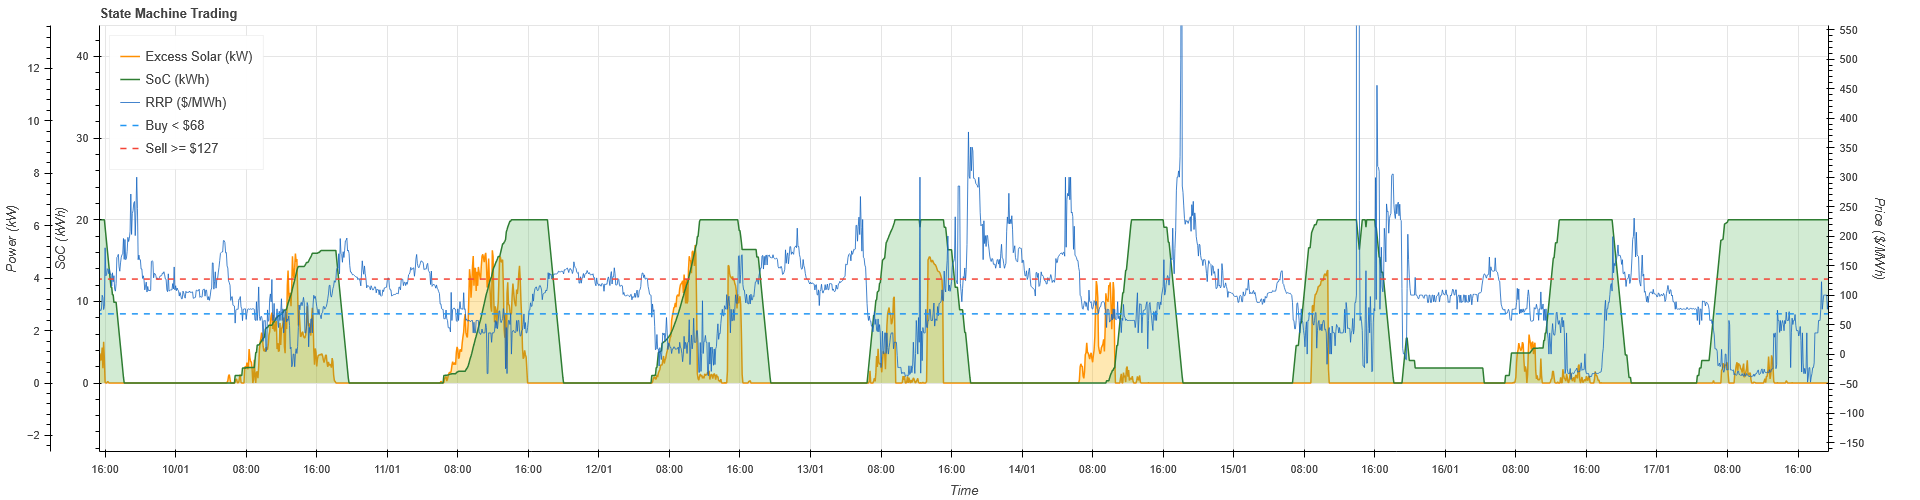
\includegraphics[width=1\textwidth]{images/statemachine_week.png}
    \caption{One week period of state machine control January 2025}
    \label{fig:statemachine_result}
\end{figure}

Figure~\ref{fig:sm_rrp_percentile} provides insight into the pricing events that are contributing most to the export revenue generated. Figure~\ref{fig:sm_rrp_percentile_99-100} shows that exports during the top 0.1\% of dispatch intervals by price, the nine intervals at or above \$1510/MWh, contribute 52.5\% of total export revenue over the month. The battery orchestration exported during all nine of these intervals. This distribution of revenue highlights the importance of capturing peak pricing events. It additionally raises questions about how to future-proof a trading system where price peaks become less common as greater commercial BESS capacity is brought online.

\begin{figure}[H]
    \centering
    \begin{subfigure}[b]{0.48\textwidth}
        \centering
        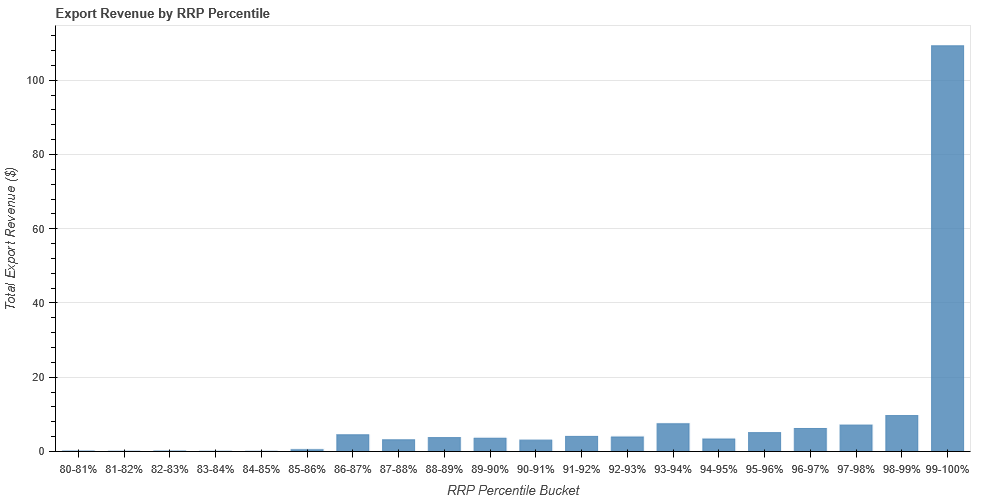
\includegraphics[width=\textwidth]{images/statemachine_rrp_percentile.png}
        \caption{80-100th percentile}
        \label{fig:sm_rrp_percentile_80-100}
    \end{subfigure}
    \hfill
    \begin{subfigure}[b]{0.48\textwidth}
        \centering
        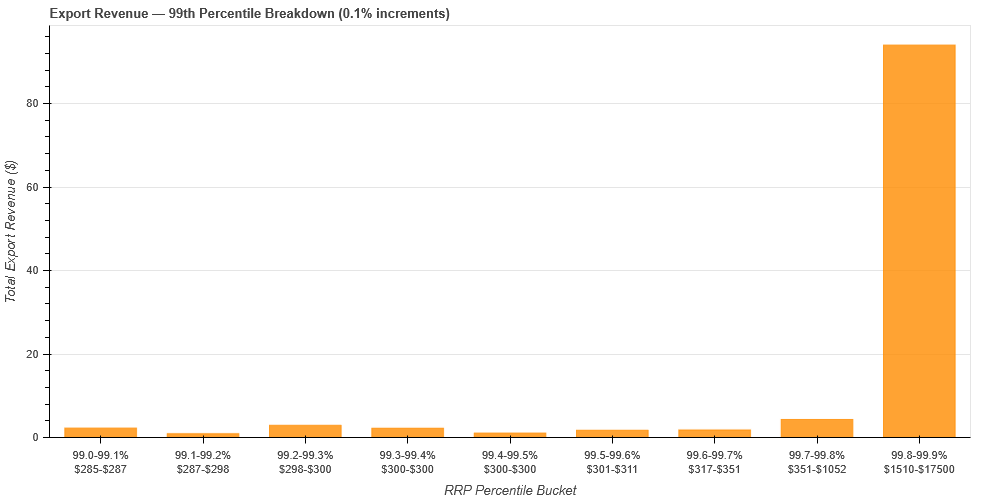
\includegraphics[width=\textwidth]{images/statemachine_rrp_percentile_99_.png}
        \caption{99-100th percentile}
        \label{fig:sm_rrp_percentile_99-100}
    \end{subfigure}
    \caption{Export revenue by dispatch period RRP percentile}
    \label{fig:sm_rrp_percentile}
\end{figure}

% -----------------------------------------------------------------------------
% Spot-trading results. Numbers come from code/trading/results/*.csv;
% code/trading/RESULTS.md is the source text.
%
% STALE (2026-09-21): the meter data was re-stamped to interval end, which moves the
% household series by one 5-min interval against the price series. The state machine,
% perfect-foresight MILP, export limit and retail numbers are on the corrected data,
% with the no-battery spot reference at -91.80. The forecast study (Tables
% tab:mpc:headline and tab:mpc:bands, the text of Section sec:results:mpc, and the
% LSTM / seasonal-naive rows and the spike-excluded LSTM figures in the comparison
% section) is still from the old join, where the reference was -91.31 and perfect
% foresight returned 28.74 rather than 28.25. Refresh with
%     cd code/trading && python forecast_trading.py        (about 1 hour)
% and re-read results/forecast_summary.csv and results/mpc_household_J4_*.csv.
% -----------------------------------------------------------------------------

\section{Genie Model}
Establishes an upper bound of to measure the effect of cycling age cost

\subsection{Upper Bound Results}
Result that sets the upper bound for our further study


\subsection{Battery Degredation Model}
Ignoring degreadation removes the value of trading. 

The MILP was solved with a rolling horizon: each window covers 48~hours, the first
24~hours are committed, and the per-segment energy is carried into the next window,
giving 31 windows for the month. Two scenarios were run. In the \emph{household}
scenario the battery sits behind the meter with the solar and load. In the
\emph{battery-only} scenario the household terms are zero and the battery trades alone.
Results are given in Tables~\ref{tab:milp:household} and~\ref{tab:milp:bess}.

\begin{table}[htbp]
    \centering
    \small
    \caption{Perfect-foresight MILP, household scenario, January 2025. Error is the
    relative difference between the degradation cost inside the MILP and the rainflow
    cost. The state machine uses thresholds of \$69.70 and \$127.20 per MWh on a 20~kWh
    lossless battery and is included for qualitative comparison only.}
    \label{tab:milp:household}
    \begin{tabular}{@{}lrrrrrr@{}}
        \toprule
        Model & \shortstack{Profit\\at meter (\$)} & \shortstack{Rainflow\\deg.\ (\$)} &
        \shortstack{Net\\profit (\$)} & \shortstack{Life\\lost (\%)} &
        \shortstack{Full\\cycles} & \shortstack{Error\\(\%)} \\
        \midrule
        $J=1$, $R^{\mathrm{cell}}=0$ & 95.04 & 194.62 & $-99.58$ & 1.622 & 42.4 & -- \\
        $J=1$  & 14.40 & 2.40  & 12.00 & 0.020 & 1.0  & 170 \\
        $J=2$  & 43.52 & 22.61 & 20.91 & 0.188 & 8.0  & 15.4 \\
        $J=4$  & 43.31 & 15.07 & 28.25 & 0.126 & 9.3  & 4.1 \\
        $J=8$  & 47.69 & 16.86 & 30.83 & 0.141 & 12.7 & 0.9 \\
        $J=16$ & 48.62 & 16.67 & 31.95 & 0.139 & 15.0 & 3.9 \\
        \midrule
        State machine & 53.16 & 136.70 & $-83.53$ & 1.139 & 25.6 & -- \\
        \bottomrule
    \end{tabular}
\end{table}

\begin{table}[htbp]
    \centering
    \small
    \caption{Perfect-foresight MILP, battery-only scenario, January 2025.}
    \label{tab:milp:bess}
    \begin{tabular}{@{}lrrrrr@{}}
        \toprule
        Model & \shortstack{Profit\\at meter (\$)} & \shortstack{Rainflow\\deg.\ (\$)} &
        \shortstack{Net\\profit (\$)} & \shortstack{Full\\cycles} & \shortstack{Error\\(\%)} \\
        \midrule
        $J=1$, $R^{\mathrm{cell}}=0$ & 136.23 & 139.31 & $-3.09$ & 25.4 & -- \\
        $J=1$  & 103.98 & 1.68 & 102.30 & 0.9 & 252 \\
        $J=2$  & 105.91 & 2.94 & 102.98 & 1.4 & 51 \\
        $J=4$  & 113.97 & 6.77 & 107.20 & 4.8 & 12.5 \\
        $J=8$  & 113.41 & 5.22 & 108.19 & 5.0 & 6.9 \\
        $J=16$ & 113.55 & 5.16 & 108.39 & 5.4 & 2.6 \\
        \bottomrule
    \end{tabular}
\end{table}

\paragraph{Ignoring degradation removes the value of trading.}
With $R^{\mathrm{cell}} = 0$ the optimiser earns the most at the meter, \$95.04 in the
household scenario and \$136.23 for the battery alone, but it completes 42 and 25
equivalent full cycles in the month and consumes 1.6\% and 1.2\% of the battery's cycle
life. Once that wear is valued by rainflow counting, both scenarios make a net loss. The
threshold state machine fails in the same way: it earns more at the meter than any
degradation-aware MILP and loses all of it to aging, for a net result of $-$\$83.53.

\paragraph{A degradation-aware controller trades about a fifth as often and keeps the profit.}
At $J = 4$ the household battery completes 9.3 equivalent full cycles, loses 0.126\% of
its life, and returns a net profit of \$28.25. Relative to the no-battery position this
is \$120.04 of value added after \$15.07 of aging.


\section{Price Forecasters}

\subsection{Seasonal Naive}

\subsection{AEMO Pre-Dispatch}

\subsection{LSTM}


\section{Net-Demand Forecasters}
\subsection{7-Day Load Profile}

\subsection{LSTM}

\section{Spot trading and retail comparison}
\label{sec:results:trading}

This chapter reports three studies carried out on the battery model of
Chapter~\ref{ch:systemmodel}.
The first solves the mixed-integer linear program (MILP) with perfect foresight to
establish an upper bound and to measure the effect of the cycle-aging cost. The second
replaces perfect foresight with forecasts inside a model predictive control (MPC) loop,
and measures how much of that upper bound a realisable controller recovers. The third
operates the same battery for self-consumption on a set-rate retail tariff, as a
reference for what a household would obtain without market exposure.

\subsection{Common setup}
\label{sec:results:setup}

All results are for the 31 days of January 2025 in the NSW1 region, which is 8928
five-minute dispatch intervals. All monetary values are in Australian dollars for that
month.

% STALE (2026-10-03): the battery was changed from the Powerwall 3 (13.5 kWh usable,
% eta = 0.943, R_cell = $12 000) to the generic battery of Table 3.1 described below.
% Every number in this chapter and in the analysis chapter is from the old parameters.
% Re-run python milp_trading.py, forecast_trading.py and retail_trading.py, then refresh.
The battery is the generic lithium-ion battery of Table~\ref{tab:battery_params}, with a
rated capacity of 13.5~kWh operated between 15\% and 95\% state of charge, a
maximum charge power of 5~kW, a maximum discharge power of 11.04~kW, charge and
discharge efficiencies of $\eta_c = \eta_d = 0.95$, and an initial energy of
$E_0 = 6.75$~kWh. The household is a single dwelling with rooftop solar. Its meter
records import and export only, so the model observes the net local power
$G_n - A_n$ and never $G_n$ and $A_n$ separately. The meter registers both an import
and an export in 636 of the intervals. The two channels are netted within each
interval in every study in this chapter, including the no-battery references, because
the dispatch models see only the net. On that basis the household without a battery
imports 458~kWh and exports 490~kWh over the month (464~kWh and 495~kWh on the raw
channels).

Under spot settlement, imported energy is charged at the spot price plus the network
tariff, $R_n + N$ with $N = 10.80$~c/kWh \cite{ausgrid2024networkpricelist},
and exported energy is paid the spot price $R_n$. Battery degradation is represented
inside the MILP by the $J$-segment cycle-aging cost of Xu et al.~\cite{Xu2018}.
Every dispatch schedule is additionally valued after the fact by rainflow cycle counting,
using the stress function $\Phi(\delta) = 5.24\times10^{-4}\,\delta^{2.03}$ and a cell
replacement cost of $R^{\mathrm{cell}} = \$10\,800$ (\$800/kWh). Throughout this chapter, \emph{net
profit} means profit at the meter less the rainflow degradation cost, so that schedules
produced with different values of $J$ are valued on the same basis.

The spot price in January 2025 had a mean of \$83/MWh and a median of \$76/MWh. It was
negative in 15.2\% of intervals, above \$300/MWh in 0.45\% of intervals, and above
\$1000/MWh in ten intervals, which fell on 1, 14, 15 and 22 January. The maximum was the
market price cap of \$17\,500/MWh on 15 January.



% -----------------------------------------------------------------------------


\paragraph{Four segments are sufficient.}
With a single segment, all cycling is priced at one marginal cost and the battery barely
trades. Net profit rises steeply up to $J = 4$ and then flattens: \$28.25, \$30.83 and
\$31.95 at $J = 4$, 8 and 16, for solve times of 12~s, 27~s and 59~s. At $J = 4$ the
degradation cost inside the MILP agrees with the rainflow cost to within 4.1\%. The
error is not monotonic in $J$ beyond this point (0.9\% at $J = 8$ and 3.9\% at
$J = 16$). The error is an absolute value and its sign changes: the MILP overstates the
rainflow cost at $J = 4$ and $J = 8$ and understates it at $J = 16$. Below about 5\% the
error is therefore no longer controlled by the number of segments. The cause has not
been isolated; the candidates are the 24-hour commitment of a 48-hour window, the
terminal constraint applied to every window, and the solver optimality gap. $J = 4$ is
used for the forecasting study as the smallest value at which the error is below 5\%.



\paragraph{Co-located solar and load increase the value of the battery.}
Before aging, the battery adds \$135.11 in the household scenario against \$113.97 when
trading alone. This is consistent with the battery charging from surplus solar that
would otherwise be exported at $R_n$, and discharging into load that would otherwise be
imported at $R_n + N$, so that it earns the network tariff in addition to the price
spread.

% -----------------------------------------------------------------------------
\subsection{Forecast-driven dispatch}
\label{sec:results:mpc}

This study measures the \emph{dispatch value} of a forecast: the net profit obtained
when the MILP plans on that forecast, compared with the net profit under perfect
foresight. The household scenario is used with $J = 4$.

At every five-minute interval the controller solves the MILP over a 24-hour horizon,
implements the first interval only, and repeats, giving 8928 solves per forecaster at
0.14 to 0.33~s each. Following the information structure of
Chapter~\ref{ch:systemmodel}, the price of the current interval is known, because AEMO
publishes it before the interval begins, while all later prices and all net local power,
including that of the current interval, are forecast. The implemented charge and
discharge powers are then settled against the actual price and the actual net local
power.

Three price forecasters are compared. Each issues a forecast of the mean price in each
of the next 48 half-hours, which is held constant across the six dispatch intervals of
the half-hour.
\begin{itemize}
    \item \emph{Seasonal naive}: the mean price of the same half-hour on the previous
    day.
    \item \emph{AEMO pre-dispatch}: the regional price from the most recent AEMO
    pre-dispatch run published at or before the start of the interval, with
    intervention runs excluded. A run extends to the end of the next trading day, which
    can be less than 24~hours ahead, and the remainder of the horizon is filled with the
    seasonal-naive forecast.
    \item \emph{LSTM}: a two-layer LSTM with 64 hidden units and a dropout of 0.2 reads
    the previous seven days (336 half-hours) of price, regional demand and calendar
    features (sine and cosine of the time of day, day of week and day of year). Its
    final hidden state is concatenated with the calendar features of the 48 target
    half-hours and passed through a fully connected layer of 128 units to produce all
    48 forecasts at once. Prices are transformed by $\sinh^{-1}(R/100)$, which is
    approximately linear near zero, logarithmic for large prices and defined for
    negative prices, and demand is standardised. The network is trained with a Huber
    loss on the transformed prices using Adam with a learning rate of $10^{-3}$ and a
    batch size of 256, on 2015 to 2023, with early stopping on the 2024 validation
    loss. A forecast is issued at the start of every half-hour from data up to the end
    of the previous half-hour.
\end{itemize}
The literature behind these choices is reviewed in Section~\ref{sub:forecast:price}.
The net local power is forecast in every case by the mean of the same five-minute slot
over the previous seven days, which has a mean absolute error of 1.15~kW. The
\emph{perfect price} case uses actual prices with this household forecast, and so
separates the cost of the household forecast from the cost of the price forecast.

\begin{table}[htbp]
    \centering
    \small
    \caption{Forecast accuracy and dispatch value, household scenario, $J=4$, January
    2025. MAE is the mean absolute error of the price forecast over all lead times and
    rMAE is the MAE relative to the seasonal-naive forecast.}
    \label{tab:mpc:headline}
    \begin{tabular}{@{}lrrrrrrr@{}}
        \toprule
        Forecaster & \shortstack{MAE\\(\$/MWh)} & \shortstack{Median\\AE} & rMAE &
        \shortstack{Profit\\at meter (\$)} & \shortstack{Rainflow\\deg.\ (\$)} &
        \shortstack{Net\\profit (\$)} & \shortstack{\% of\\perfect} \\
        \midrule
        Perfect                  & 0     & 0    & --   & 43.85 & 15.11 & 28.74 & 100 \\
        Perfect price            & 0     & 0    & --   & 34.33 & 14.69 & 19.64 & 68 \\
        LSTM                     & 44.6  & 22.0 & 0.73 & 33.29 & 17.35 & 15.94 & 55 \\
        Seasonal naive           & 61.3  & 25.3 & 1.00 & 31.71 & 15.79 & 15.92 & 55 \\
        AEMO pre-dispatch        & 161.6 & 16.4 & 2.63 & 30.24 & 15.57 & 14.67 & 51 \\
        \bottomrule
    \end{tabular}
\end{table}

On the 2024 validation year the LSTM had an MAE of \$70.3/MWh against \$103.1/MWh for
the seasonal-naive forecast, an rMAE of 0.68, with the best model obtained at epoch 5.
January 2025 was not used for training or model selection.

\paragraph{The rolling loop costs nothing under perfect information.}
Perfect foresight on the 24-hour, five-minute MPC loop gives the same net profit as the
48-hour rolling solve to within one cent (\$28.74), although the two schedules differ in
4\% of intervals. Every gap in Table~\ref{tab:mpc:headline} is therefore caused by
forecast error and not by the horizon or the re-planning frequency.

\paragraph{Most of the loss comes from the household forecast, not the price forecast.}
Knowing every price but forecasting the net local power loses \$9.10 of the
\$12.80 to \$14.07 total gap. Measured against the perfect-price case, the price
forecasts cost \$3.70 for the LSTM, \$3.72 for the seasonal-naive forecast and \$4.97
for AEMO pre-dispatch.

\paragraph{A more accurate price forecast did not produce more dispatch value.}
The LSTM reduces the MAE by 27\% relative to the seasonal-naive forecast, from
\$61.3/MWh to \$44.6/MWh, and finishes two cents ahead of it. It earns \$1.59 more at
the meter, but its schedule has deeper cycles (a mean depth of 0.196 against 0.158) and
incurs \$1.56 more in aging.



\paragraph{AEMO pre-dispatch is the most accurate forecast in normal conditions and the least accurate on average.}
It has the lowest median error (\$16.4/MWh) and the highest MAE (\$161.6/MWh). It
forecast prices near the market price cap on the hot days of 14--15 and 21--22 January
that largely did not eventuate: 1.0\% of its forecast values exceed \$1000/MWh, against
0.1\% of actual prices. With every forecast value capped at \$1000/MWh before the error
is taken, its MAE is \$48.9/MWh, between the LSTM (\$44.7/MWh) and the seasonal-naive
forecast (\$53.2/MWh). Actual prices are not capped in this measure, so a perfect
forecast scores \$11.6/MWh on it. In dispatch it finishes \$1.25 below the seasonal-naive forecast.

\paragraph{Forecast accuracy and dispatch value are only loosely related.}
Ranked by MAE the order is LSTM, seasonal naive, AEMO pre-dispatch. Ranked by net
profit the LSTM and the seasonal-naive forecast are level and AEMO pre-dispatch is
slightly behind, with all three within \$1.27 of one another.


\subsubsection{Implications}
\label{sec:results:mpc:implications}

The assumption that carries the most weight in this study is that the price of the
current interval is known before the dispatch decision is made. It is what secures the
\$101.53 earned during price spikes. The assumption is realistic, but its value has not
yet been measured, and doing so requires only that the study be repeated with the
current-interval price forecast rather than observed.

The spike revenue was captured because the battery was not empty when each spike
arrived. One month containing four spike days is not evidence that a controller will
generally hold charge at the right time. A reserve state of charge, or a
spike-probability input, would address that risk. It would not close the \$12.80 gap
measured here, because that gap does not arise from spikes.

The largest recoverable loss is the household forecast, at \$9.10. An improved forecast
of net local power is worth more than any further improvement to the price model. Part
of this loss is a property of the controller and not of the forecast. The loop commits a
battery power for the whole interval from a forecast of the net local power, and the
forecast is a seven-day mean that does not use the most recent meter readings, although
Chapter~\ref{ch:systemmodel} makes them available. A battery inverter measures the net
load continuously, so a controller that committed a grid power target, or that
corrected the forecast with the latest readings, would recover some of the \$9.10
without a better day-ahead forecast.

% -----------------------------------------------------------------------------
\subsection{Retail self-consumption}
\label{sec:results:retail}

As a reference for a household without market exposure, the same battery was operated
for self-consumption on two published AGL Residential Smart Saver plans for the Ausgrid
network area \cite{AGLSmartSaver}, % TODO: verify plan details against the source document
both with a feed-in tariff of 3.0~c/kWh. The single-rate plan charges 29.82~c/kWh with a
supply charge of 149.57~c/day. The time-of-use plan charges 54.18~c/kWh from 3~pm to
9~pm and 21.63~c/kWh otherwise, with a supply charge of 158.63~c/day. The retail rates
include GST.

Two controllers are compared on each plan. The \emph{self-consumption rule} charges from
surplus solar, discharges into household load, and never exchanges energy with the grid
on the battery's behalf. On a single-rate tariff with no export limit this rule is
optimal before aging, since the import rate exceeds the feed-in rate at every instant.
It has no price signal against which to weigh a cycle, so its aging is only valued after
the fact by rainflow counting. The rule has no terminal constraint, so it is started
from the state of charge that the same rule reaches at the end of December, which is
empty, and it also ends January empty. The \emph{optimised} controller is the MILP of
Chapter~\ref{ch:systemmodel} with the import and export rates of the plan in place of
$R_n + N$ and $R_n$, the same $J = 4$ aging cost, perfect foresight of the net local
power, and the same 48-hour rolling horizon, initial energy and terminal constraint as
Section~\ref{sec:results:milp}. It is the like-for-like counterpart of the
perfect-foresight spot result: the same optimiser and aging cost on different prices.
It may charge from the grid, which is only worthwhile on the time-of-use plan.

\begin{table}[htbp]
    \centering
    \small
    \caption{Retail plans, January 2025 (\$). The bill without a battery is \$168.21 on
    the single-rate plan and \$196.53 on the time-of-use plan.}
    \label{tab:retail}
    \begin{tabular}{@{}llrrrrrr@{}}
        \toprule
        Plan & Controller & \shortstack{Bill with\\battery} & \shortstack{Gross\\saving} &
        \shortstack{Rainflow\\deg.} & \shortstack{Net\\saving} & \shortstack{Life\\lost (\%)} &
        \shortstack{Full\\cycles} \\
        \midrule
        Single rate & Self-consumption rule & 112.27 & 55.94 & 63.36 & $-7.42$ & 0.528 & 15.7 \\
        Single rate & Optimised, $J=4$      & 138.01 & 30.20 & 12.38 & 17.82   & 0.103 & 8.5 \\
        Time of use & Self-consumption rule & 125.32 & 71.21 & 63.36 & 7.85    & 0.528 & 15.7 \\
        Time of use & Optimised, $J=4$      & 134.93 & 61.61 & 25.47 & 36.14   & 0.212 & 11.1 \\
        \bottomrule
    \end{tabular}
\end{table}

The dispatch of the rule is identical on both plans, because it does not depend on
price. Grid import falls from 458~kWh to 246~kWh and export from 490~kWh to 252~kWh,
with 15.7 equivalent full cycles and 0.53\% of cycle life consumed.

The household is better off on the single-rate plan with or without the battery. The
choice of plan is worth \$28 in the month without a battery, which is half of the gross
saving of the rule on that plan. The battery is nevertheless worth more on the
time-of-use plan under either controller, because the imports it displaces are more
expensive there. The supply charge is 28\% of the single-rate bill and cannot be reduced
by storage, so on that plan the battery earns only on the 26.82~c/kWh difference between
the usage rate and the feed-in tariff.

The rule has the larger gross saving and the smaller net saving on both plans. It cycles
on every solar surplus regardless of the cost of doing so, consumes 0.53\% of cycle life
in the month, about four times the 0.126\% of degradation-aware spot trading, and on the
single-rate plan its gross saving does not cover the modelled aging cost. The optimised
controller gives up \$10 to \$26 of gross saving, avoids \$38 to \$51 of aging, and
returns a positive net saving on both plans. The negative result of the rule is therefore
a property of the controller under this aging cost, not of the retail tariff.

% -----------------------------------------------------------------------------


